%-----------------------------------LICENSE------------------------------------%
%   This file is part of tikz_figures.                                         %
%                                                                              %
%   tikz_figures is free software: you can redistribute it and/or              %
%   modify it it under the terms of the GNU General Public License as          %
%   published by the Free Software Foundation, either version 3 of the         %
%   License, or (at your option) any later version.                            %
%                                                                              %
%   tikz_figures is distributed in the hope that it will be useful,            %
%   but WITHOUT ANY WARRANTY; without even the implied warranty of             %
%   MERCHANTABILITY or FITNESS FOR A PARTICULAR PURPOSE.  See the              %
%   GNU General Public License for more details.                               %
%                                                                              %
%   You should have received a copy of the GNU General Public License along    %
%   with tikz_figures.  If not, see <https://www.gnu.org/licenses/>.           %
%------------------------------------------------------------------------------%

% Use the standalone class for displaying the tikz image on a small PDF.
\documentclass[crop, tikz]{standalone}

% Import the tikz package to use for the drawing.
\usepackage{tikz}

% Used for the LaTeX arrow.
\usetikzlibrary{arrows.meta}

% Draw angles and add labels to them.
\usetikzlibrary{
    angles, % Drawing angles within triangles.
    quotes  % Adding labels to angles.
}

% Begin the document.
\begin{document}

    % Begin the drawing.
    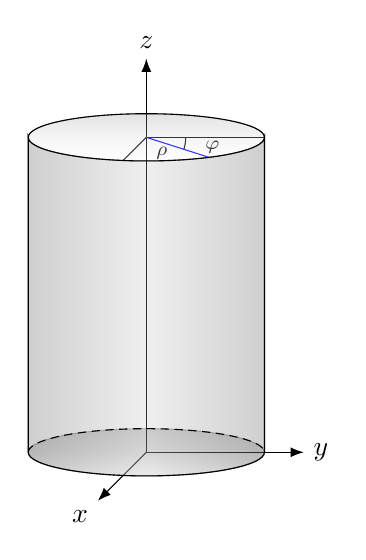
\begin{tikzpicture}[>=Latex]

        % Points for the drawing.
        \coordinate (O) at (0.0, 0.0, 0.0);
        \coordinate (x) at (0.0, 0.0, 1.6);
        \coordinate (y) at (2.0, 0.0, 0.0);
        \coordinate (z) at (0.0, 5.0, 0.0);
        \coordinate (xt) at (0.0, 4.0, 0.76);
        \coordinate (yt) at (1.5, 4.0, 0.0);
        \coordinate (zt) at (0.0, 4.0, 0.0);
        \coordinate (p) at (1.05, 4.0, 0.66);

        % Defining points for the cylinder.
        \coordinate (C0) at (1.5, 0.0);
        \coordinate (C1) at (1.5, 4.0);
        \coordinate (C2) at (-1.5, 0.0);

        % Draw the coordinate axes.
        \draw[->] (O) to (x) node[below left] {$x$};
        \draw[->] (O) to (y) node[right] {$y$};
        \draw[->] (O) to (z) node[above] {$z$};

        % Draw the upper x and y coordinate axes in the cylinder.
        \draw (zt) to (xt);
        \draw (zt) to (yt);

        % Blue line representing the radial direction on the cylinder.
        \draw[draw = blue] (zt) node [below right] {\scriptsize{$\rho$}} to (p);

        % Circle arc for the azimuthal angle, labeled phi.
        \pic[%
            draw = black,
            "\scriptsize{${\varphi}$}",
            angle eccentricity = 1.7,
            angle radius = 0.5cm
        ] {angle = p--zt--yt};

        % Fill in the bottom part of the cylinder using a filled circle.
        \draw[%
            top color = gray!50!black,
            bottom color = gray!10,
            middle color = gray,
            shading = axis,
            opacity = 0.25
        ] (0.0, 0.0) circle (1.5 and 0.3);

        % Fill in the vertical part of the cylinder as well.
        \draw[%
            left color = gray!50!black,
            right color = gray!50!black,
            middle color = gray!50,
            shading = axis,
            opacity = 0.25
        ] (C0) to (C1) arc (360:180:1.5cm and 0.3cm)
               to (C2) arc (180:360:1.5cm and 0.3cm) to cycle;

        % Fill in the top part of the cylinder using a circle.
        \draw[%
            top color = gray!90!,
            bottom color = gray!2,
            middle color = gray!30,
            shading = axis,
            opacity = 0.25
        ] (0.0, 4.0) circle (1.5cm and 0.3cm);

        % Fill in the outline of the cylinder.
        \draw (C0) to (C1) arc (360:180:1.5cm and 0.3cm)
                   to (C2) arc (180:360:1.5cm and 0.3cm) to cycle;

        \draw (-1.5, 4.0) arc (180:0:1.5cm and 0.3cm);
        
        % The last part is the back-side, so make it dashed to indicate this.
        \draw[densely dashed] (-1.5, 0.0) arc (180:0:1.5cm and 0.3cm);
    \end{tikzpicture}
\end{document}
